\section{INTRODUCTION}
\begin{frame} % First frame
    \frametitle{Context: hardware security}
%    \framesubtitle{Context}

%    \begin{itemize}
%        \setlength\itemsep{1em}
%        \item Electronics systems are found in every sector;
%        \item IoT, CPS, bank electronics → embed cryptographic protocols to ensure secure operation;
%%        \item These implementations are fallible → they leak information.
%    \end{itemize}
%
%    \begin{figure}
%        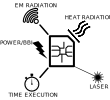
\includegraphics[width=0.4\textwidth]{chipCard.pdf}
%        \caption{Side-channel and fault injection.}
%    \end{figure}

    \begin{columns}
        \begin{column}{0.6\textwidth}
            \begin{itemize}
                \item Electronics are found in every economic sector;
                \item In IoT, CPS, debit cards, phones, bank systems;
                \item They embed cryptographic algorithms to ensure security;
                \item These algorithms are fallible, they leak data and can be disturbed.
            \end{itemize}
        \end{column}

        \barsep

        \begin{column}{0.4\textwidth}
            \begin{figure}
                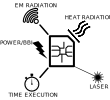
\includegraphics[width=1.0\textwidth]{chipCard.pdf}
                \caption{Side-channel and fault injection.}
            \end{figure}
        \end{column}
    \end{columns}

%    \begin{columns}
%        \begin{column}{0.3\textwidth}
%            \centering
%            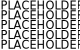
\includegraphics[width=\textwidth]{8by9_PLACEHOLDER.pdf}
%        \end{column}
%
%        \begin{column}{0.3\textwidth}
%            \centering
%            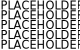
\includegraphics[width=\textwidth]{8by9_PLACEHOLDER.pdf}
%        \end{column}
%    \end{columns}

    %        \begin{center}
        %            Jeaj
        %        \end{center}
\end{frame}